\documentclass[]{book}
\usepackage{lmodern}
\usepackage{amssymb,amsmath}
\usepackage{ifxetex,ifluatex}
\usepackage{fixltx2e} % provides \textsubscript
\ifnum 0\ifxetex 1\fi\ifluatex 1\fi=0 % if pdftex
  \usepackage[T1]{fontenc}
  \usepackage[utf8]{inputenc}
\else % if luatex or xelatex
  \ifxetex
    \usepackage{mathspec}
  \else
    \usepackage{fontspec}
  \fi
  \defaultfontfeatures{Ligatures=TeX,Scale=MatchLowercase}
\fi
% use upquote if available, for straight quotes in verbatim environments
\IfFileExists{upquote.sty}{\usepackage{upquote}}{}
% use microtype if available
\IfFileExists{microtype.sty}{%
\usepackage{microtype}
\UseMicrotypeSet[protrusion]{basicmath} % disable protrusion for tt fonts
}{}
\usepackage[margin=1in]{geometry}
\usepackage{hyperref}
\hypersetup{unicode=true,
            pdftitle={A Minimal Book Example},
            pdfauthor={Sergio},
            pdfborder={0 0 0},
            breaklinks=true}
\urlstyle{same}  % don't use monospace font for urls
\usepackage{natbib}
\bibliographystyle{apalike}
\usepackage{color}
\usepackage{fancyvrb}
\newcommand{\VerbBar}{|}
\newcommand{\VERB}{\Verb[commandchars=\\\{\}]}
\DefineVerbatimEnvironment{Highlighting}{Verbatim}{commandchars=\\\{\}}
% Add ',fontsize=\small' for more characters per line
\usepackage{framed}
\definecolor{shadecolor}{RGB}{248,248,248}
\newenvironment{Shaded}{\begin{snugshade}}{\end{snugshade}}
\newcommand{\KeywordTok}[1]{\textcolor[rgb]{0.13,0.29,0.53}{\textbf{#1}}}
\newcommand{\DataTypeTok}[1]{\textcolor[rgb]{0.13,0.29,0.53}{#1}}
\newcommand{\DecValTok}[1]{\textcolor[rgb]{0.00,0.00,0.81}{#1}}
\newcommand{\BaseNTok}[1]{\textcolor[rgb]{0.00,0.00,0.81}{#1}}
\newcommand{\FloatTok}[1]{\textcolor[rgb]{0.00,0.00,0.81}{#1}}
\newcommand{\ConstantTok}[1]{\textcolor[rgb]{0.00,0.00,0.00}{#1}}
\newcommand{\CharTok}[1]{\textcolor[rgb]{0.31,0.60,0.02}{#1}}
\newcommand{\SpecialCharTok}[1]{\textcolor[rgb]{0.00,0.00,0.00}{#1}}
\newcommand{\StringTok}[1]{\textcolor[rgb]{0.31,0.60,0.02}{#1}}
\newcommand{\VerbatimStringTok}[1]{\textcolor[rgb]{0.31,0.60,0.02}{#1}}
\newcommand{\SpecialStringTok}[1]{\textcolor[rgb]{0.31,0.60,0.02}{#1}}
\newcommand{\ImportTok}[1]{#1}
\newcommand{\CommentTok}[1]{\textcolor[rgb]{0.56,0.35,0.01}{\textit{#1}}}
\newcommand{\DocumentationTok}[1]{\textcolor[rgb]{0.56,0.35,0.01}{\textbf{\textit{#1}}}}
\newcommand{\AnnotationTok}[1]{\textcolor[rgb]{0.56,0.35,0.01}{\textbf{\textit{#1}}}}
\newcommand{\CommentVarTok}[1]{\textcolor[rgb]{0.56,0.35,0.01}{\textbf{\textit{#1}}}}
\newcommand{\OtherTok}[1]{\textcolor[rgb]{0.56,0.35,0.01}{#1}}
\newcommand{\FunctionTok}[1]{\textcolor[rgb]{0.00,0.00,0.00}{#1}}
\newcommand{\VariableTok}[1]{\textcolor[rgb]{0.00,0.00,0.00}{#1}}
\newcommand{\ControlFlowTok}[1]{\textcolor[rgb]{0.13,0.29,0.53}{\textbf{#1}}}
\newcommand{\OperatorTok}[1]{\textcolor[rgb]{0.81,0.36,0.00}{\textbf{#1}}}
\newcommand{\BuiltInTok}[1]{#1}
\newcommand{\ExtensionTok}[1]{#1}
\newcommand{\PreprocessorTok}[1]{\textcolor[rgb]{0.56,0.35,0.01}{\textit{#1}}}
\newcommand{\AttributeTok}[1]{\textcolor[rgb]{0.77,0.63,0.00}{#1}}
\newcommand{\RegionMarkerTok}[1]{#1}
\newcommand{\InformationTok}[1]{\textcolor[rgb]{0.56,0.35,0.01}{\textbf{\textit{#1}}}}
\newcommand{\WarningTok}[1]{\textcolor[rgb]{0.56,0.35,0.01}{\textbf{\textit{#1}}}}
\newcommand{\AlertTok}[1]{\textcolor[rgb]{0.94,0.16,0.16}{#1}}
\newcommand{\ErrorTok}[1]{\textcolor[rgb]{0.64,0.00,0.00}{\textbf{#1}}}
\newcommand{\NormalTok}[1]{#1}
\usepackage{longtable,booktabs}
\usepackage{graphicx,grffile}
\makeatletter
\def\maxwidth{\ifdim\Gin@nat@width>\linewidth\linewidth\else\Gin@nat@width\fi}
\def\maxheight{\ifdim\Gin@nat@height>\textheight\textheight\else\Gin@nat@height\fi}
\makeatother
% Scale images if necessary, so that they will not overflow the page
% margins by default, and it is still possible to overwrite the defaults
% using explicit options in \includegraphics[width, height, ...]{}
\setkeys{Gin}{width=\maxwidth,height=\maxheight,keepaspectratio}
\IfFileExists{parskip.sty}{%
\usepackage{parskip}
}{% else
\setlength{\parindent}{0pt}
\setlength{\parskip}{6pt plus 2pt minus 1pt}
}
\setlength{\emergencystretch}{3em}  % prevent overfull lines
\providecommand{\tightlist}{%
  \setlength{\itemsep}{0pt}\setlength{\parskip}{0pt}}
\setcounter{secnumdepth}{5}
% Redefines (sub)paragraphs to behave more like sections
\ifx\paragraph\undefined\else
\let\oldparagraph\paragraph
\renewcommand{\paragraph}[1]{\oldparagraph{#1}\mbox{}}
\fi
\ifx\subparagraph\undefined\else
\let\oldsubparagraph\subparagraph
\renewcommand{\subparagraph}[1]{\oldsubparagraph{#1}\mbox{}}
\fi

%%% Use protect on footnotes to avoid problems with footnotes in titles
\let\rmarkdownfootnote\footnote%
\def\footnote{\protect\rmarkdownfootnote}

%%% Change title format to be more compact
\usepackage{titling}

% Create subtitle command for use in maketitle
\newcommand{\subtitle}[1]{
  \posttitle{
    \begin{center}\large#1\end{center}
    }
}

\setlength{\droptitle}{-2em}
  \title{A Minimal Book Example}
  \pretitle{\vspace{\droptitle}\centering\huge}
  \posttitle{\par}
  \author{Sergio}
  \preauthor{\centering\large\emph}
  \postauthor{\par}
  \predate{\centering\large\emph}
  \postdate{\par}
  \date{2018-02-25}

\usepackage{booktabs}
\usepackage{amsthm}
\makeatletter
\def\thm@space@setup{%
  \thm@preskip=8pt plus 2pt minus 4pt
  \thm@postskip=\thm@preskip
}
\makeatother

\usepackage{amsthm}
\newtheorem{theorem}{Theorem}[chapter]
\newtheorem{lemma}{Lemma}[chapter]
\theoremstyle{definition}
\newtheorem{definition}{Definition}[chapter]
\newtheorem{corollary}{Corollary}[chapter]
\newtheorem{proposition}{Proposition}[chapter]
\theoremstyle{definition}
\newtheorem{example}{Example}[chapter]
\theoremstyle{definition}
\newtheorem{exercise}{Exercise}[chapter]
\theoremstyle{remark}
\newtheorem*{remark}{Remark}
\newtheorem*{solution}{Solution}
\begin{document}
\maketitle

{
\setcounter{tocdepth}{1}
\tableofcontents
}
\chapter{Prerequisites}\label{prerequisites}

\begin{itemize}
\tightlist
\item
  Download and install R:

  \begin{itemize}
  \tightlist
  \item
    \url{https://cran.r-project.org/}
  \end{itemize}
\item
  Downoad and install RStudio:

  \begin{itemize}
  \tightlist
  \item
    \url{https://www.rstudio.com/products/rstudio/download/}\\
  \item
    Configure RStudio:\\
  \item
    \ldots{}
  \end{itemize}
\item
  Install R packages:

  \begin{itemize}
  \tightlist
  \item
    Devtools
  \end{itemize}
\end{itemize}

\begin{Shaded}
\begin{Highlighting}[]
\KeywordTok{install.packages}\NormalTok{(}\StringTok{"devtools"}\NormalTok{)  }
\end{Highlighting}
\end{Shaded}

\begin{verbatim}
- Bookdown (development version on GitHub)  
\end{verbatim}

\begin{Shaded}
\begin{Highlighting}[]
\NormalTok{devtools}\OperatorTok{::}\KeywordTok{install_github}\NormalTok{(}\StringTok{"rstudio/bookdown"}\NormalTok{)}
\end{Highlighting}
\end{Shaded}

\begin{verbatim}
- [Tinytex](https://yihui.name/tinytex/)  
\end{verbatim}

\begin{Shaded}
\begin{Highlighting}[]
\NormalTok{devtools}\OperatorTok{::}\KeywordTok{install_github}\NormalTok{(}\KeywordTok{c}\NormalTok{(}\StringTok{'yihui/tinytex'}\NormalTok{, }\StringTok{'rstudio/rmarkdown'}\NormalTok{))}
\NormalTok{tinytex}\OperatorTok{::}\KeywordTok{install_tinytex}\NormalTok{()}
\CommentTok{# Restart your R session and check if tinytex:::is_tinytex() is TRUE.}
\end{Highlighting}
\end{Shaded}

\begin{verbatim}
- Knitr (**NOT SURE if necessary in** ***CLEAN*** **installation**):  
\end{verbatim}

\begin{Shaded}
\begin{Highlighting}[]
\KeywordTok{install.packages}\NormalTok{(}\StringTok{'knitr'}\NormalTok{, }\DataTypeTok{dependencies =} \OtherTok{TRUE}\NormalTok{)}
\end{Highlighting}
\end{Shaded}

*If many errors appear, check it's not because you had a previous crappy
installation, \protect\hyperlink{ref_CleanPreviousCrap}{here}.

\chapter{How to minimal Bookdown}\label{how-to-minimal-bookdown}

\begin{itemize}
\tightlist
\item
  Download the
  \href{https://github.com/sergiogoro/minimal-bookdown-sergio}{minimal-bookdown-sergio}
  GitHub repository as a
  \href{https://github.com/sergiogoro/minimal-bookdown-sergio/archive/master.zip}{Zip}
  file, then unzip it locally.\\
\item
  Create a new RStudio project

  \begin{itemize}
  \tightlist
  \item
    Create a new project -\textgreater{} in existing directory
    -\textgreater{} select the local repo -\textgreater{} Create.\\
  \item
    Check: Build -\textgreater{} build book.
  \end{itemize}
\end{itemize}

If it gives this error:

\begin{Shaded}
\begin{Highlighting}[]
\OperatorTok{!}\StringTok{ }\NormalTok{Package xparse Error}\OperatorTok{:}\StringTok{ }\NormalTok{Support package l3kernel too old.}
\end{Highlighting}
\end{Shaded}

Then, update those packages from Miktex,
\href{https://tex.stackexchange.com/questions/132243/media9-l3kernel-too-old-support-outdated}{in
a special way}

\begin{enumerate}
\def\labelenumi{\arabic{enumi})}
\setcounter{enumi}{5}
\tightlist
\item
  Modificar basicos archivos (
  \url{http://seankross.com/2016/11/17/How-to-Start-a-Bookdown-Book.html}
  ) 6.1) \_output.yml 6.1.1)The only line you should change here is the
  title of the book, which in this case is A Minimal Bookdown Book
\end{enumerate}

6.2) \_bookdown.yml 6.2.1) The book\_filename field determines what the
name of the PDF and EPUB versions of your book will be called. In the
case of this book the PDF version would be bookdown-start.pdf. The
chapter\_name field is a string that is appended to the front of each
chapter heading, followed by the chapter number. Chapter headings are
designated by H1 tags in R Markdown which are usually created with a
single pound sign (\#). So for example in the file 01-Introduction.Rmd
the first H1 tag is \# Introduction which becomes �Chapter 1
Introduction� when the book is rendered. The repo field just designates
a GitHub repository associated with this book but this is not a required
field. The output\_dir field determines the directory where the HTML
files for your book will be rendered. If you don�t set this field your
book will be rendered in a directory called \_book/, however if you�re
going to be sharing your book with GitHub Pages I highly recommend
specifying the docs directory for output\_dir. GitHub Pages has a new
feature which allows you to use a docs/ folder in the master branch of
your repo to publish a static website. This allows you to track the
source files for your book and the published HTML files in the same
branch, eliminating the need for that pesky gh-pages branch. The
rmd\_files field is optional. If it is not specified then all Rmd files
at the root of your book directory are rendered as chapters in your
book. Alternatively you can list the files you want to be rendered like
I have in \_bookdown.yml. The new\_session field is also optional. If
you specify new\_session: yes then each Rmd file is rendered in its own
R session, otherwise all Rmd files in your book are rednered in the same
R session.

6.3) index.Rmd 6.3.1) This file serves as the cover and first few pages
of your book, so authors usually put the Preface and/or the Introduction
in this file. At the top of this file is a slice of yaml frontmatter
that looks like this: --- title: ``A Minimal Bookdown Book'' author:
``Sean Kross'' date: ``2016-12-02'' site: bookdown::bookdown\_site
documentclass: book bibliography: {[}book.bib{]} biblio-style: apalike
link-citations: yes github-repo: seankross/bookdown-start url:
`http://seankross.com/bookdown-start/' description: ``Everything you
need (and nothing more) to start a bookdown book.'' --- You should
change the title, author, date, github-repo, url, and description fields
to customize your book. I omitted a field called cover-image where you
can specify the path to a image file for the cover of your book (I know
.png works for sure).

\begin{enumerate}
\def\labelenumi{\arabic{enumi})}
\setcounter{enumi}{6}
\item
  Escribir, editando los archivos desde Rstudio (u otro editor) Once you
  have those three configuration flies set up writing a bookdown book
  couldn�t be easier if you�re familiar with R Markdown. Just write Rmd
  files in the root directory of your book (where index.Rmd is) and run
  bookdown::render\_book(``index.Rmd'') periodically to compile your
  book. You can preview the book by opening up the index.html file in
  the directory where your book is rendered (docs/index.html in the case
  of bookdown-start). It�s also good practice to name your Rmd files so
  that they�re ordered, which you can see I�ve done with the prefixes of
  01-, 02-, etc. You can then publish the book on GitHub Pages or you
  can upload the book to bookdown.org with the publish\_book() function.
\item
  Compilar libro desde RStudio 8.1)
  bookdown::render\_book(``index.Rmd'') 8.2) Abrir
  ``repolocal''/docs/index.html
\end{enumerate}

\hypertarget{ref_CleanPreviousCrap}{\chapter{Clean previous
crap}\label{ref_CleanPreviousCrap}}

\begin{itemize}
\tightlist
\item
  If there was a dirty installation of packages,
  \href{https://www.r-bloggers.com/how-to-remove-all-user-installed-packages-in-r/}{remove
  all user installed packages in R} (caution!):
\end{itemize}

\begin{verbatim}
# create a list of all installed packages
 ip <- as.data.frame(installed.packages())
 head(ip)
# if you use MRO, make sure that no packages in this library will be removed
 ip <- subset(ip, !grepl("MRO", ip$LibPath))
# we don't want to remove base or recommended packages either\
 ip <- ip[!(ip[,"Priority"] %in% c("base", "recommended")),]
# determine the library where the packages are installed
 path.lib <- unique(ip$LibPath)
# create a vector with all the names of the packages you want to remove
 pkgs.to.remove <- ip[,1]
 head(pkgs.to.remove)
# remove the packages
 sapply(pkgs.to.remove, remove.packages, lib = path.lib)
\end{verbatim}

\begin{itemize}
\tightlist
\item
  If installed various latex shits, they are under:
\end{itemize}

\begin{Shaded}
\begin{Highlighting}[]
\NormalTok{C}\OperatorTok{:}\NormalTok{\textbackslash{}Users\textbackslash{}}\OperatorTok{$}\NormalTok{USER\textbackslash{}AppData\textbackslash{}Local\textbackslash{}Programs\textbackslash{}MiKTeX }\FloatTok{2.9}
\NormalTok{C}\OperatorTok{:}\NormalTok{\textbackslash{}Users\textbackslash{}}\OperatorTok{$}\NormalTok{USER\textbackslash{}AppData\textbackslash{} somewhere here is the tinytex dir.}
\end{Highlighting}
\end{Shaded}

\chapter{Introduction}\label{intro}

You can label chapter and section titles using \texttt{\{\#label\}}
after them, e.g., we can reference Chapter \ref{intro}. If you do not
manually label them, there will be automatic labels anyway, e.g.,
Chapter \ref{methods}.

Figures and tables with captions will be placed in \texttt{figure} and
\texttt{table} environments, respectively.

\begin{Shaded}
\begin{Highlighting}[]
\KeywordTok{par}\NormalTok{(}\DataTypeTok{mar =} \KeywordTok{c}\NormalTok{(}\DecValTok{4}\NormalTok{, }\DecValTok{4}\NormalTok{, .}\DecValTok{1}\NormalTok{, .}\DecValTok{1}\NormalTok{))}
\KeywordTok{plot}\NormalTok{(pressure, }\DataTypeTok{type =} \StringTok{'b'}\NormalTok{, }\DataTypeTok{pch =} \DecValTok{19}\NormalTok{)}
\end{Highlighting}
\end{Shaded}

\begin{figure}

{\centering 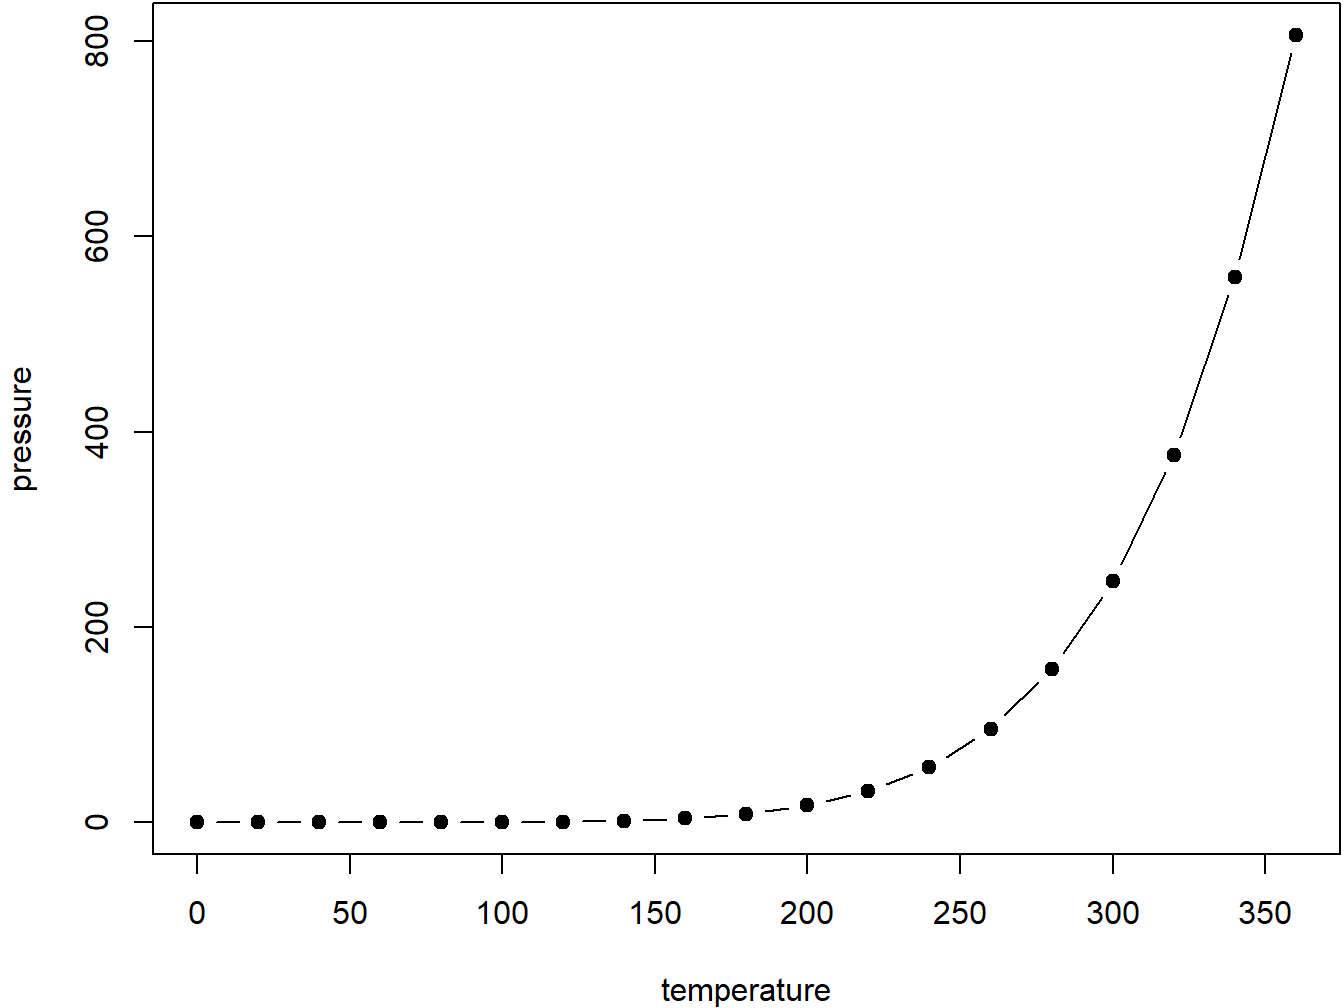
\includegraphics[width=0.8\linewidth]{minimal-bookdown-sergio_files/figure-latex/nice-fig-1} 

}

\caption{Here is a nice figure!}\label{fig:nice-fig}
\end{figure}

Reference a figure by its code chunk label with the \texttt{fig:}
prefix, e.g., see Figure \ref{fig:nice-fig}. Similarly, you can
reference tables generated from \texttt{knitr::kable()}, e.g., see Table
\ref{tab:nice-tab}.

\begin{Shaded}
\begin{Highlighting}[]
\NormalTok{knitr}\OperatorTok{::}\KeywordTok{kable}\NormalTok{(}
  \KeywordTok{head}\NormalTok{(iris, }\DecValTok{20}\NormalTok{), }\DataTypeTok{caption =} \StringTok{'Here is a nice table!'}\NormalTok{,}
  \DataTypeTok{booktabs =} \OtherTok{TRUE}
\NormalTok{)}
\end{Highlighting}
\end{Shaded}

\begin{table}

\caption{\label{tab:nice-tab}Here is a nice table!}
\centering
\begin{tabular}[t]{rrrrl}
\toprule
Sepal.Length & Sepal.Width & Petal.Length & Petal.Width & Species\\
\midrule
5.1 & 3.5 & 1.4 & 0.2 & setosa\\
4.9 & 3.0 & 1.4 & 0.2 & setosa\\
4.7 & 3.2 & 1.3 & 0.2 & setosa\\
4.6 & 3.1 & 1.5 & 0.2 & setosa\\
5.0 & 3.6 & 1.4 & 0.2 & setosa\\
\addlinespace
5.4 & 3.9 & 1.7 & 0.4 & setosa\\
4.6 & 3.4 & 1.4 & 0.3 & setosa\\
5.0 & 3.4 & 1.5 & 0.2 & setosa\\
4.4 & 2.9 & 1.4 & 0.2 & setosa\\
4.9 & 3.1 & 1.5 & 0.1 & setosa\\
\addlinespace
5.4 & 3.7 & 1.5 & 0.2 & setosa\\
4.8 & 3.4 & 1.6 & 0.2 & setosa\\
4.8 & 3.0 & 1.4 & 0.1 & setosa\\
4.3 & 3.0 & 1.1 & 0.1 & setosa\\
5.8 & 4.0 & 1.2 & 0.2 & setosa\\
\addlinespace
5.7 & 4.4 & 1.5 & 0.4 & setosa\\
5.4 & 3.9 & 1.3 & 0.4 & setosa\\
5.1 & 3.5 & 1.4 & 0.3 & setosa\\
5.7 & 3.8 & 1.7 & 0.3 & setosa\\
5.1 & 3.8 & 1.5 & 0.3 & setosa\\
\bottomrule
\end{tabular}
\end{table}

You can write citations, too. For example, we are using the
\textbf{bookdown} package \citep{R-bookdown} in this sample book, which
was built on top of R Markdown and \textbf{knitr} \citep{xie2015}.

\bibliography{book.bib,packages.bib}


\end{document}
